% Svolgimento: prova del 14/09/2021, esercizio 3 (catalogo B65-E03).
% Quesito teorico: pressione totale e urto obliquo. Numeri e figure da calcoli.py.

\documentclass[11pt,a4paper]{article}

\usepackage[T1]{fontenc}
\usepackage[utf8]{inputenc}
\usepackage[italian]{babel}
\usepackage{amsmath,amssymb}
\usepackage[a4paper,margin=2.5cm]{geometry}
\usepackage{array}

\usepackage{siunitx}
\usepackage{booktabs}
\usepackage{graphicx}
\usepackage{float}
\usepackage{hyperref}

\hypersetup{hidelinks}
\setlength{\parindent}{0pt}
\setlength{\parskip}{4pt}
\allowdisplaybreaks
\graphicspath{{figure/}}

\sisetup{output-decimal-marker={,}, group-separator={\,}, per-mode=symbol,
         exponent-product=\cdot, range-phrase={\text{--}}}

\newcommand{\Vv}{\boldsymbol V}
\newcommand{\sth}{s_{\rm th}}
\newcommand{\Mn}{M_{n1}}
\newcommand{\kk}{\frac{\gamma}{\gamma-1}}
\newcommand{\Mr}{M_{r}}

\title{Gasdinamica -- Svolgimento \texttt{B65-E03}\\[2pt]
\large Pressione totale e urto obliquo}
\author{}
\date{Prova del 14/09/2021, esercizio 3}

\begin{document}
\maketitle

\section*{Traccia}
\begin{center}
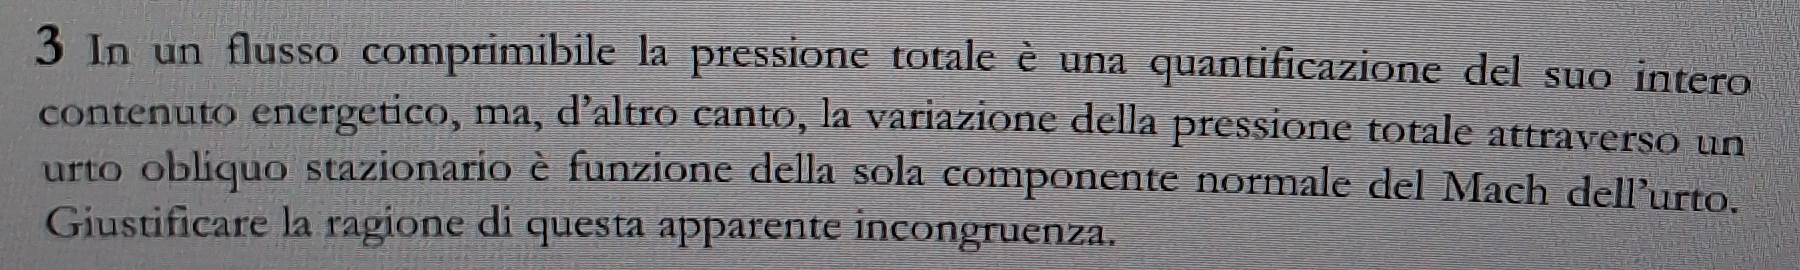
\includegraphics[width=0.95\textwidth]{traccia_es3.png}
\end{center}
In un flusso comprimibile la pressione totale è una quantificazione del suo intero contenuto energetico, ma,
d'altro canto, la variazione della pressione totale attraverso un urto obliquo stazionario è funzione della sola
componente normale del Mach dell'urto. Giustificare la ragione di questa apparente incongruenza.

%==============================================================================
\section{Lettura del testo e dati}
È un quesito teorico: non ci sono dati e la risposta è un ragionamento. Il testo accosta due affermazioni:
\begin{enumerate}
  \item[(A)] la pressione totale $p_0$ quantifica \emph{tutto} il contenuto energetico della corrente, quindi
    dipende sia dall'energia interna sia dall'energia cinetica, con \emph{entrambe} le componenti della velocità;
  \item[(B)] attraverso un urto obliquo stazionario la variazione di $p_0$ dipende solo da
    $\Mn=M_1\sin\sigma$, cioè non dalla componente tangenziale della velocità.
\end{enumerate}
Va spiegato perché (B) non contraddice (A). Per ``variazione'' intendo, come nelle relazioni d'urto, il rapporto
$p_{0,2}/p_{0,1}$; alla fine discuto anche la differenza $p_{0,1}-p_{0,2}$, che si comporta diversamente.

Per gli esempi numerici uso aria, $\gamma=\num{1.4}$ ($\delta=\num{0.2}$), e $M_1=5$, lo stesso Mach dell'esercizio~2
della prova, con un angolo d'urto tale che $\Mn=2$.

%==============================================================================
\section{Modello e ipotesi}
\begin{itemize}
  \item \textbf{Eulero 2D stazionario}, gas perfetto a $\gamma$ costante: è il modello in cui è definito l'urto
    obliquo stazionario della traccia.
  \item \textbf{Urto piano} di spessore nullo tra due stati uniformi 1 (monte) e 2 (valle). Per un urto curvo il
    ragionamento vale punto per punto, con il $\sigma$ locale.
  \item \textbf{Nessuno scambio di calore né lavoro con l'esterno}: l'urto è fermo, quindi non compie lavoro sul
    fluido. Questa ipotesi è quella che rende costante l'entalpia totale e va tenuta presente quando si cambia
    riferimento.
  \item \textbf{Pressione totale} secondo la definizione del corso: la pressione che la particella raggiunge
    se viene portata in quiete con una trasformazione isentropica,
    \[
      \frac{T_0}{T}=1+\delta M^2,\qquad
      \frac{p_0}{p}=\left(\frac{T_0}{T}\right)^{\kk}=\left(1+\delta M^2\right)^{\kk}.
    \]
    $p_0$ dipende dal modulo della velocità, quindi dal riferimento in cui la si misura; $p$, $\rho$, $T$ e
    l'entropia no.
\end{itemize}

%==============================================================================
\section{Analisi qualitativa}
L'apparente contraddizione nasce dal significato attribuito a $p_0$. Il \emph{contenuto energetico} per unità di
massa di una corrente stazionaria è l'entalpia totale $h_0=c_pT_0=h+|\Vv|^2/2$, e attraverso l'urto fermo
$h_0$ \textbf{si conserva}: l'urto non toglie energia alla corrente. Scrivendo la definizione di $p_0$ rispetto a un
qualunque stato di riferimento (r) e usando
$\Delta\sth=c_p\ln(T/T_r)-R\ln(p/p_r)$, si ottiene
\[
  p_0=p_r\left(\frac{T_0}{T_r}\right)^{\kk}\exp\!\left(-\frac{\sth-s_{\rm th,r}}{R}\right):
\]
$p_0$ contiene due informazioni, il \emph{livello} dell'energia ($T_0$) e la sua \emph{qualità} (l'entropia).
La seconda è quella che conta per l'uso dell'energia: la massima velocità ottenibile espandendo la corrente fino a
una pressione $p_b$ è
\[
  V^2=2c_pT_0\left[1-\left(\frac{p_b}{p_0}\right)^{\frac{\gamma-1}{\gamma}}\right],
\]
quindi, a pari $T_0$, una $p_0$ minore vuol dire meno energia trasformabile in energia cinetica o in lavoro. In
questo senso $p_0$ quantifica l'``intero contenuto energetico'': ne misura la parte utilizzabile.

Attraverso l'urto $T_0$ non cambia, dunque la variazione di $p_0$ misura \textbf{solo la produzione di entropia}.
L'entropia è una grandezza termodinamica, uguale per ogni osservatore, e l'urto è una compressione che avviene
\emph{solo nella direzione normale} al fronte: la velocità tangenziale lo attraversa invariata, senza gradienti e
senza compressione. Mi aspetto quindi che il rapporto $p_{0,2}/p_{0,1}$ dipenda solo da $\Mn$, mentre l'energia
cinetica tangenziale compaia in $p_{0,1}$ e in $p_{0,2}$ nella stessa misura e si semplifichi nel rapporto.

%==============================================================================
\section{Topologia del campo}
Lo stato uniforme 1, con $M_1$ e direzione $\theta_1=0$, incontra l'urto obliquo piano inclinato di $\sigma$
sulla velocità di monte; a valle c'è lo stato uniforme 2, deviato di $\theta$ verso l'urto. La velocità si
scompone rispetto al fronte (fig.~\ref{fig:rif}a) in una componente normale $V_n$ e una tangenziale $V_t$:
\[
  V_{n1}=|\Vv_1|\sin\sigma,\qquad V_{t1}=|\Vv_1|\cos\sigma,\qquad
  \Mn=M_1\sin\sigma,\qquad M_{t1}=M_1\cos\sigma .
\]
Lo stesso campo si può guardare da un osservatore che scorre lungo l'urto con velocità $V_t$
(fig.~\ref{fig:rif}b). Poiché si muove \emph{parallelamente} al fronte, per lui l'urto resta fermo e il campo
resta stazionario.

%==============================================================================
\section{Bilancio equazioni/incognite}
Noti lo stato 1 e $\sigma$, le incognite dello stato 2 sono quattro: $\rho_2$, $V_{n2}$, $V_{t2}$, $p_2$. Le
equazioni sono le quattro relazioni di salto scritte nel riferimento ruotato con l'urto (massa, quantità di moto
normale e tangenziale, energia):
\[
  [\rho V_n]=0,\qquad [p+\rho V_n^2]=0,\qquad [\rho V_n V_t]=0,\qquad
  \left[\rho V_n\Big(h+\frac{V_n^2+V_t^2}{2}\Big)\right]=0 .
\]
Il problema è chiuso, e si spezza in due. Con $\rho V_n\neq0$ (urto, non linea di scorrimento) la terza dà
$[V_t]=0$: la componente tangenziale si conserva e non entra nelle altre equazioni, perché il termine
$V_t^2/2$ è uguale ai due lati e si elide dall'energia. Restano
\[
  [\rho V_n]=0,\qquad [p+\rho V_n^2]=0,\qquad \Big[h+\frac{V_n^2}{2}\Big]=0,
\]
che sono \emph{esattamente} le relazioni di Rankine--Hugoniot di un urto normale con velocità di monte $V_{n1}$.
Lo stato termodinamico a valle dipende quindi solo dallo stato 1 e da $\Mn$.

%==============================================================================
\section{Scorciatoie fisiche}
Lo stesso risultato si legge con il cambio di riferimento galileiano. Le equazioni di Eulero non cambiano
passando a un riferimento in moto uniforme; cambiano solo le velocità, non $p$, $\rho$, $T$ e l'entropia.
L'osservatore che scorre con $V_t$ vede un \textbf{urto normale} con Mach di monte $\Mn$
(fig.~\ref{fig:rif}b), quindi
\[
  \frac{p_2}{p_1},\ \frac{\rho_2}{\rho_1},\ \frac{T_2}{T_1},\ \Delta\sth
  \quad\text{sono quelle dell'urto normale a } \Mn .
\]
Non sono invece invarianti $M$, $T_0$ e $p_0$: l'osservatore mobile misura una $p_0$ diversa da quella del
laboratorio. Resta da spiegare perché il \emph{rapporto} delle $p_0$ è lo stesso nei due riferimenti.

%==============================================================================
\section{Calcolo}
\subsection{Rapporto delle pressioni totali ed entropia}
Dalla definizione $p_0=p\,(T_0/T)^{\gamma/(\gamma-1)}$ applicata ai due lati, con $T_{0,2}=T_{0,1}$:
\[
  \frac{p_{0,2}}{p_{0,1}}=\frac{p_2}{p_1}\left(\frac{T_1}{T_2}\right)^{\kk} .
\]
Passando ai logaritmi e ricordando $\gamma/(\gamma-1)=c_p/R$ e $\Delta\sth=c_p\ln(T_2/T_1)-R\ln(p_2/p_1)$:
\[
  \boxed{\ \frac{p_{0,2}}{p_{0,1}}=\exp\!\left(-\frac{\Delta\sth}{R}\right)\ }
\]
Il rapporto delle pressioni totali è una misura della sola entropia prodotta. Con $p_2/p_1$ e $T_2/T_1$
dell'urto normale a $\Mn$ si ritrova la relazione del formulario,
\[
  \frac{p_{0,2}}{p_{0,1}}=
  \left[\frac{(\gamma+1)\Mn^2}{(\gamma-1)\Mn^2+2}\right]^{\kk}
  \left[\frac{\gamma+1}{2\gamma \Mn^2-(\gamma-1)}\right]^{\frac{1}{\gamma-1}},
\]
che contiene solo $\Mn$ e $\gamma$.

\subsection{Dove finisce l'energia cinetica tangenziale}
Separo nella temperatura totale la parte dovuta a $V_t$:
\[
  T_0=T+\frac{V_n^2}{2c_p}+\frac{V_t^2}{2c_p}=T_{0n}+\frac{V_t^2}{2c_p},
  \qquad T_{0n}:=T+\frac{V_n^2}{2c_p},
\]
dove $T_{0n}$ è la temperatura totale misurata dall'osservatore mobile. $T_0$ si conserva (energia nel
laboratorio), $V_t$ si conserva, quindi si conserva anche $T_{0n}$ (energia nel riferimento mobile): i due bilanci
sono coerenti. La pressione totale si fattorizza allo stesso modo:
\[
  p_0=p\left(\frac{T_{0n}}{T}\right)^{\kk}\left(\frac{T_0}{T_{0n}}\right)^{\kk}=p_{0n}\,C,
  \qquad C=\left(\frac{T_0}{T_{0n}}\right)^{\kk}=\left(1+\frac{V_t^2}{2c_pT_{0n}}\right)^{\kk}.
\]
$C$ dipende solo da grandezze che l'urto conserva ($T_0$, $T_{0n}$, $V_t$), quindi \textbf{è lo stesso a monte e
a valle}:
\[
  \frac{p_{0,2}}{p_{0,1}}=\frac{p_{0n,2}\,C}{p_{0n,1}\,C}=\frac{p_{0n,2}}{p_{0n,1}} .
\]
L'energia cinetica tangenziale fa parte di $p_{0,1}$ e di $p_{0,2}$, e le moltiplica per lo stesso fattore: è
contata in entrambe, ma nel rapporto si elide.

\subsection{Variazione assoluta}
La differenza delle pressioni totali, invece, è
\[
  p_{0,1}-p_{0,2}=p_{0,1}\left[1-\frac{p_{0,2}}{p_{0,1}}(\Mn)\right],\qquad
  \frac{p_{0,1}}{p_1}=\left(1+\delta M_1^2\right)^{\kk},
\]
e dipende da tutto $M_1$ attraverso $p_{0,1}$: la perdita assoluta è proporzionale all'intero contenuto energetico,
la sua frazione dipende solo da $\Mn$.

\subsection{Esempio numerico}
Con $M_1=5$ e $\Mn=2$:
\[
  \sigma=\arcsin\frac{\Mn}{M_1}=\ang{23.6},\qquad \theta=\ang{14.3},\qquad M_2=\num{3.57},
\]
\[
  \frac{p_2}{p_1}=\num{4.50},\qquad \frac{T_2}{T_1}=\num{1.69},\qquad
  \frac{V_{n1}}{V_{n2}}=\frac{\rho_2}{\rho_1}=\num{2.67},\qquad V_{t2}=V_{t1}.
\]
Nel laboratorio $T_0/T_1=6$ e $p_{0,1}/p_1=529$; per l'osservatore mobile $T_{0n}/T_1=\num{1.8}$ e
$p_{0n,1}/p_1=\num{7.82}$. Il fattore comune vale $C=\num{67.6}$, e
\[
  \frac{p_{0,2}}{p_{0,1}}=\frac{p_{0n,2}}{p_{0n,1}}=\num{0.721},\qquad
  \frac{\Delta\sth}{R}=\num{0.327} .
\]
La tabella~\ref{tab:conf} confronta questo urto obliquo con l'urto normale allo stesso $\Mn$ e con quello
allo stesso $M_1$.

\begin{table}[H]
  \centering\small
  \setlength{\tabcolsep}{4pt}
  \begin{tabular}{lccccccc}
    \toprule
    Caso & $\Mn$ & $p_2/p_1$ & $T_2/T_1$ & $p_{0,1}/p_1$ & $p_{0,2}/p_{0,1}$ & $(p_{0,1}-p_{0,2})/p_1$ &
    $\Delta\sth/R$ \\
    \midrule
    normale, $M_1=2$             & 2 & \num{4.50} & \num{1.69} & \num{7.82} & \num{0.721} & \num{2.18} & \num{0.327} \\
    obliquo, $M_1=5$           & 2 & \num{4.50} & \num{1.69} & 529 & \num{0.721} & 148 & \num{0.327} \\
    normale, $M_1=5$             & 5 & 29 & \num{5.80} & 529 & \num{0.0617} & 496 & \num{2.79} \\
    \bottomrule
  \end{tabular}
  \caption{Stesso $\Mn$: stesse grandezze termodinamiche e stesso rapporto delle $p_0$, perdita assoluta
  diversa. Stesso $M_1$: perdita molto diversa a seconda di $\sigma$.}
  \label{tab:conf}
\end{table}

%==============================================================================
\section{Verifiche a posteriori}
\begin{itemize}
  \item Caso $\sigma=\ang{90}$: $\Mn=M_1$ e si ritrova l'urto normale. Verificata.
  \item Caso $\sigma\to\mu$: $\Mn\to1$, $p_{0,2}/p_{0,1}\to1$ (onda di Mach). Il salto d'entropia va a zero come
    $\Delta\sth/R\simeq\frac{2\gamma}{3(\gamma+1)^2}(\Mn^2-1)^3$, del terzo ordine come atteso per un urto debole.
    Verificata.
  \item Segno: $\Delta\sth>0$ e $p_{0,2}<p_{0,1}$ se e solo se $\Mn>1$; per $\Mn<1$ sarebbe un urto di
    espansione, impossibile. Verificata.
  \item Conservazione dell'energia: $T_{0,2}=T_{0,1}$ nel laboratorio e $T_{0n,2}=T_{0n,1}$ nel riferimento mobile.
    Verificata.
  \item Invarianza galileiana: $p_2/p_1$, $\rho_2/\rho_1$ e $p_{0,2}/p_{0,1}$ coincidono nei due riferimenti
    (tabella, righe 1 e 2), e $V_{t2}=V_{t1}$. Verificata.
  \item Modello 2D stazionario: lo stato 2 dell'esempio è supersonico ($M_2=\num{3.57}$, ramo debole). Verificata.
\end{itemize}

%==============================================================================
\section{Risultati}
\begin{itemize}
  \item $p_0$ dipende da due cose: il livello di energia $T_0$, che attraverso l'urto stazionario si conserva, e
    l'entropia. Il rapporto delle pressioni totali misura quindi \textbf{solo l'entropia prodotta},
    $p_{0,2}/p_{0,1}=\exp(-\Delta\sth/R)$: l'urto non distrugge energia, ne degrada la qualità.
  \item L'entropia è una grandezza termodinamica, uguale per ogni osservatore. Per un osservatore che scorre
    lungo il fronte con $V_t$ l'urto obliquo è un urto normale a $\Mn$, quindi $\Delta\sth$ dipende solo da $\Mn$.
  \item L'energia cinetica tangenziale attraversa l'urto invariata: compare in $p_{0,1}$ e in $p_{0,2}$ come lo
    stesso fattore $C=(T_0/T_{0n})^{\gamma/(\gamma-1)}$ e si elide nel rapporto. Non c'è quindi incongruenza: $p_0$
    contiene tutta l'energia, ma la sua \emph{variazione relativa} misura solo la parte processata dall'urto.
  \item La perdita assoluta $p_{0,1}-p_{0,2}$ dipende invece anche da $M_1$, tramite $p_{0,1}$.
\end{itemize}

%==============================================================================
\section{Rappresentazioni}
\begin{figure}[H]
  \centering
  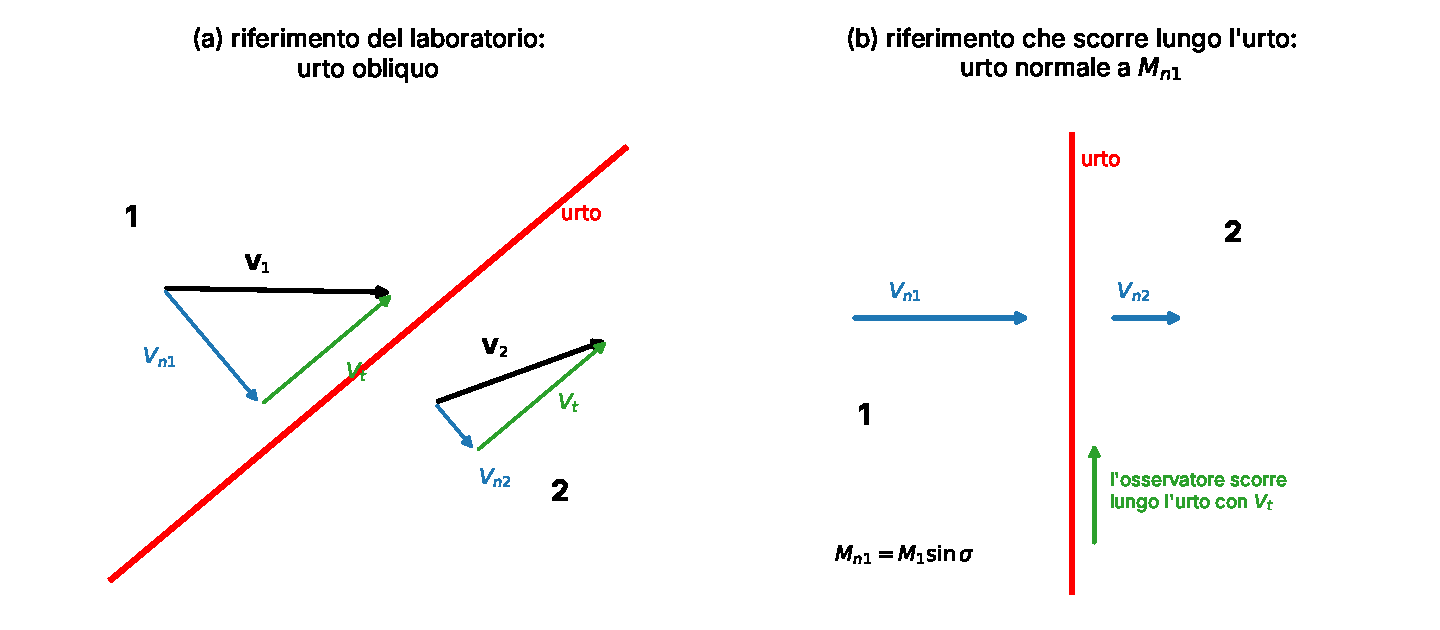
\includegraphics[width=0.95\textwidth]{riferimenti.pdf}
  \caption{Lo stesso urto in due riferimenti (proporzioni qualitative). (a) Laboratorio: la componente tangenziale
  $V_t$ si conserva, la normale si riduce da $V_{n1}$ a $V_{n2}$ e la corrente devia verso l'urto. (b) Osservatore
  che scorre lungo il fronte con $V_t$: urto normale con Mach di monte $\Mn$.}
  \label{fig:rif}
\end{figure}
La figura~\ref{fig:rif} mostra la scomposizione della velocità. Nel laboratorio la deviazione $\theta$ nasce solo
dal fatto che $V_n$ diminuisce mentre $V_t$ resta uguale; togliendo $V_t$ a entrambi gli stati resta un urto
normale, con gli stessi $p$, $\rho$, $T$ ai due lati.

\begin{figure}[H]
  \centering
  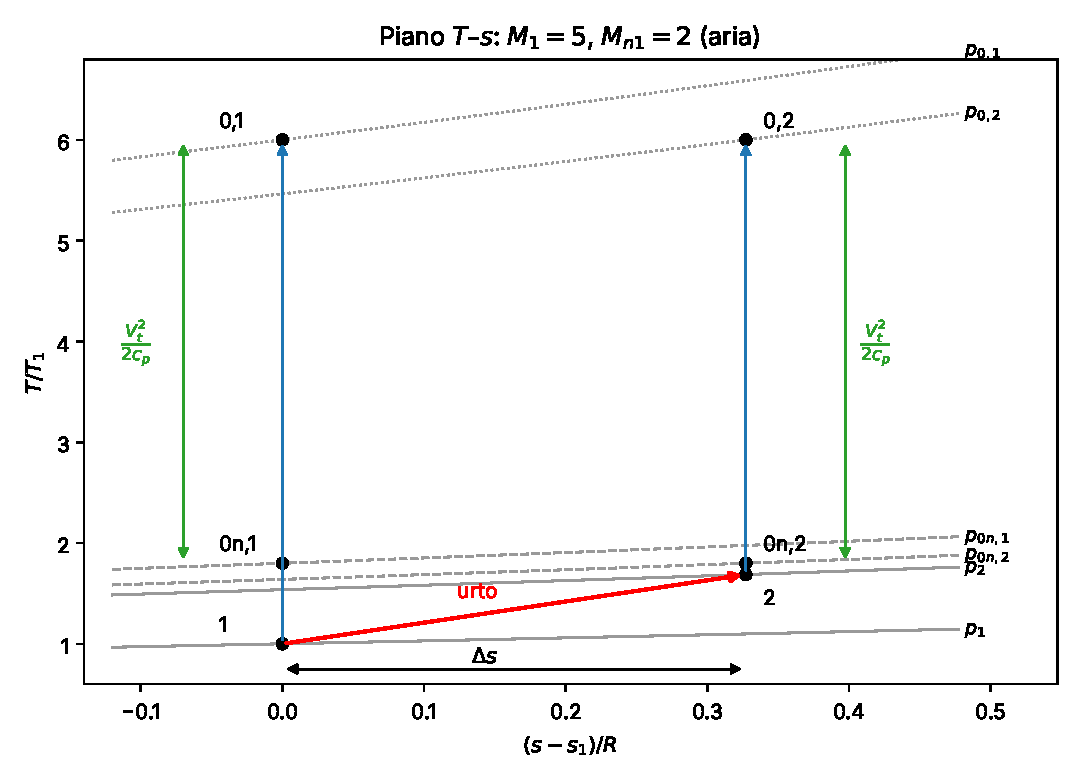
\includegraphics[width=0.72\textwidth]{piano_Ts.pdf}
  \caption{Piano $T$--$s$ per $M_1=5$, $\Mn=2$: stati statici 1 e 2, stati di ristagno nel laboratorio
  ($0,1$ e $0,2$) e per l'osservatore mobile ($0n,1$ e $0n,2$), con le rispettive isobare.}
  \label{fig:Ts}
\end{figure}
La figura~\ref{fig:Ts} è la rappresentazione più diretta della risposta. L'urto porta da 1 a 2 con un aumento
di entropia $\Delta s$; i ristagni isentropici sono segmenti verticali. Gli stati di ristagno del laboratorio stanno
a $T_0$, quelli dell'osservatore mobile a $T_{0n}$, più in basso della stessa quantità $V_t^2/(2c_p)$ da entrambi i
lati. In un gas perfetto due isobare a una data temperatura distano $\Delta s$ con rapporto di pressione
$\exp(\Delta s/R)$, \emph{a qualunque temperatura}: per questo il rapporto $p_{0,2}/p_{0,1}$ letto a $T_0$ coincide
con $p_{0n,2}/p_{0n,1}$ letto a $T_{0n}$, anche se le pressioni totali sono molto diverse ($529$ contro $\num{7.8}$
volte $p_1$).

\begin{figure}[H]
  \centering
  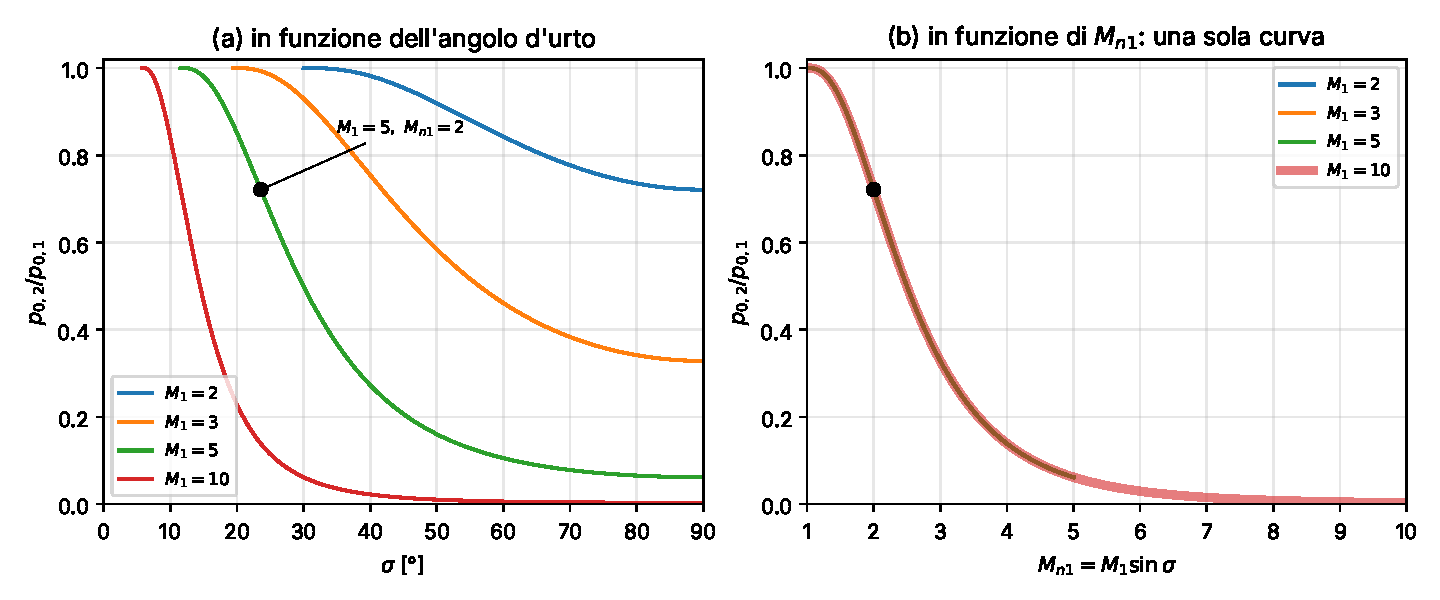
\includegraphics[width=0.95\textwidth]{rapporto_p0.pdf}
  \caption{$p_{0,2}/p_{0,1}$ per $M_1=2,3,5,10$: (a) in funzione di $\sigma$, da $\mu$ a \ang{90}; (b) in
  funzione di $\Mn=M_1\sin\sigma$. Il punto è l'esempio $M_1=5$, $\Mn=2$.}
  \label{fig:rapp}
\end{figure}
Nella figura~\ref{fig:rapp}a le curve partono da $p_{0,2}/p_{0,1}=1$ all'angolo di Mach e scendono fino al valore
dell'urto normale a $\sigma=\ang{90}$, diverso per ogni $M_1$. Riportate in funzione di $\Mn$ (fig.~\ref{fig:rapp}b)
\emph{collassano su un'unica curva}, quella dell'urto normale: è l'affermazione (B) della traccia in forma grafica.

\begin{figure}[H]
  \centering
  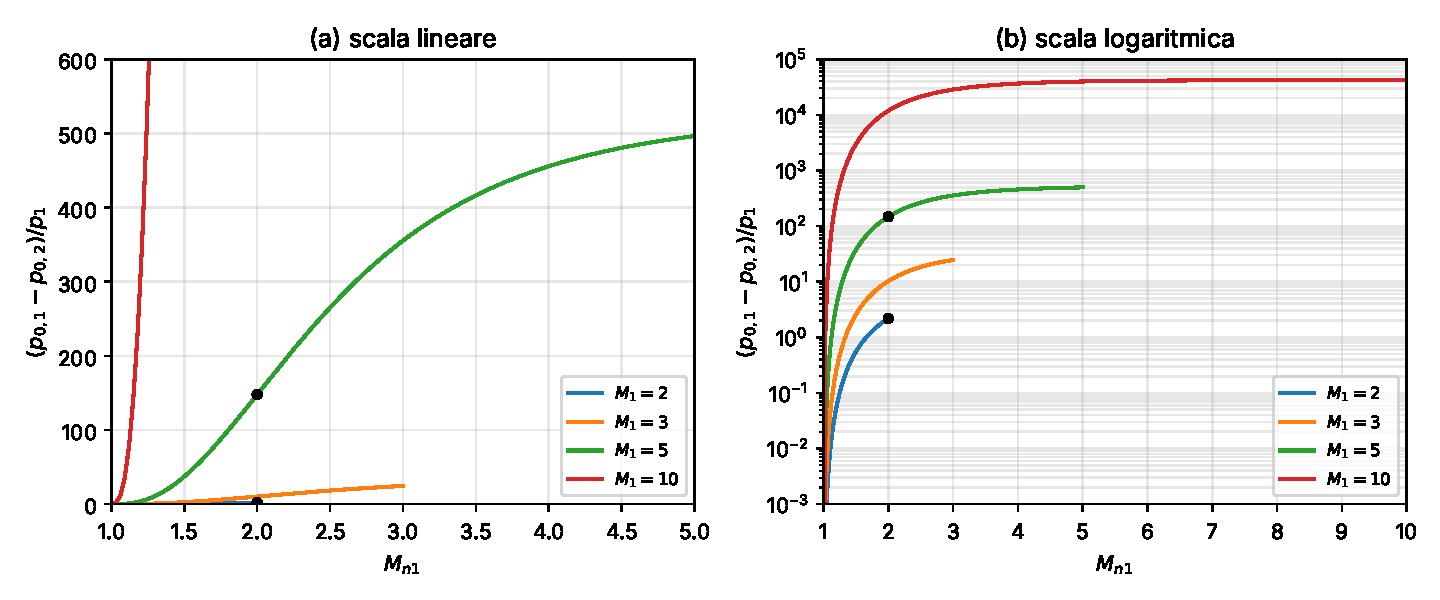
\includegraphics[width=0.95\textwidth]{perdita_assoluta.pdf}
  \caption{Perdita assoluta $(p_{0,1}-p_{0,2})/p_1$ in funzione di $\Mn$, per $M_1=2,3,5,10$: (a) scala lineare,
  (b) scala logaritmica. I punti sono i primi due casi della tabella~\ref{tab:conf} ($\Mn=2$).}
  \label{fig:ass}
\end{figure}
La perdita assoluta (fig.~\ref{fig:ass}) non collassa: a pari $\Mn$ cresce con $M_1$ come $p_{0,1}$, cioè con
tutto il contenuto energetico. I valori vanno da quasi zero a decine di migliaia di volte $p_1$: la scala lineare
mostra bene la crescita per $M_1=5$ ma schiaccia i casi $M_1=2$ e $3$ sull'asse; la scala logaritmica li rende
leggibili tutti e mostra che le curve sono la stessa curva traslata verticalmente di $\log p_{0,1}$,
proprio perché la frazione persa è la stessa.

%==============================================================================
\section{Discussione fisica}
\textbf{Perché solo la direzione normale.} L'entropia si produce dentro lo spessore dell'urto, per viscosità e
conduzione, cioè dove ci sono gradienti. Lungo la normale $V_n$ e $T$ variano bruscamente; $V_t$ invece è uguale ai
due lati e la quantità di moto tangenziale non ha motivo di variare all'interno: non ci sono sforzi di taglio né
dissipazione legata a $V_t$. L'energia cinetica tangenziale è solo trasportata, come se l'urto non ci fosse.

\textbf{Conseguenza progettuale.} A pari $M_1$, la perdita dipende dall'inclinazione dell'urto: un urto obliquo,
con $\Mn$ piccolo, dissipa molto meno di un urto normale. Per esempio, a $M_1=5$ un urto normale conserva solo
$p_{0,2}/p_{0,1}=\num{0.062}$; due rampe da \ang{11} e un urto normale finale (a $M=\num{3.14}$) ne conservano
$\num{0.22}$, più di tre volte tanto. È il principio delle prese d'aria supersoniche a più urti obliqui e del
fatto che a bassi $\Mn$ la compressione per urto è praticamente isentropica, dato che $\Delta\sth$ va come
$(\Mn^2-1)^3$.

\textbf{Urto curvo.} Lungo un bow shock $\sigma$ varia da \ang{90} (urto normale davanti al ristagno) a $\mu$
lontano dal corpo, quindi ogni linea di corrente attraversa un $\Mn$ diverso e riceve un salto di entropia e di
$p_0$ diverso, pur con $h_0$ uniforme. Il gradiente di entropia a valle genera vorticità (teorema di Crocco), e la
linea sonica non è un'isobara.

\textbf{Il ruolo della stazionarietà.} Il cambio di riferimento funziona perché l'osservatore si muove
\emph{lungo} il fronte: l'urto resta fermo, non compie lavoro, e $T_0$ si conserva in entrambi i riferimenti. Per un
urto mobile 1D le relazioni sono le stesse, con il Mach relativo $\Mr$ al posto di $\Mn$, ma solo nel riferimento
solidale all'urto. Nel riferimento del laboratorio l'urto in moto compie lavoro sul gas, $h_0$ non si conserva e il
rapporto delle $p_0$ non misura più la sola entropia: in campo instazionario $p_0$ e $h_0$ non sono grandezze
conservate.

\end{document}
